\documentclass[aspectratio=1610, english]{beamer}
\usepackage{babel}
\usepackage[utf8]{inputenc}
\usepackage{graphicx}
\usepackage{booktabs}

\mode<beamer>{
    \definecolor{links}{HTML}{2A1B81}
    \hypersetup{pdfpagemode=FullScreen, colorlinks, linkcolor=, urlcolor=links}
    \usetheme{AGH}
}

\graphicspath{{images/}}

\author[N. Kwiecien]{Natalia Kwiecien}
\title{AI Worker Burnout -- Linear Regression Analysis}
\date{}

\begin{document}
\maketitle

%-------------------------------------------------------
\begin{frame}{Outline}
    \tableofcontents
\end{frame}

%-------------------------------------------------------
\section{Dataset}

\begin{frame}{Dataset Overview}
    \begin{columns}[c]
        \column{0.35\textwidth}
        \small
        \begin{itemize}
            \item 1500 employees, 21 variables
            \item No missing values
            \item Target: \texttt{burnout\_score}
        \end{itemize}
        \vspace{0.4em}
        \textbf{Key variables:}
        \begin{itemize}
            \item \texttt{burnout\_score} (16--86)
            \item \texttt{job\_satisfaction} (1.3--5.0)
            \item \texttt{attrition\_risk}
        \end{itemize}
        \column{0.65\textwidth}
        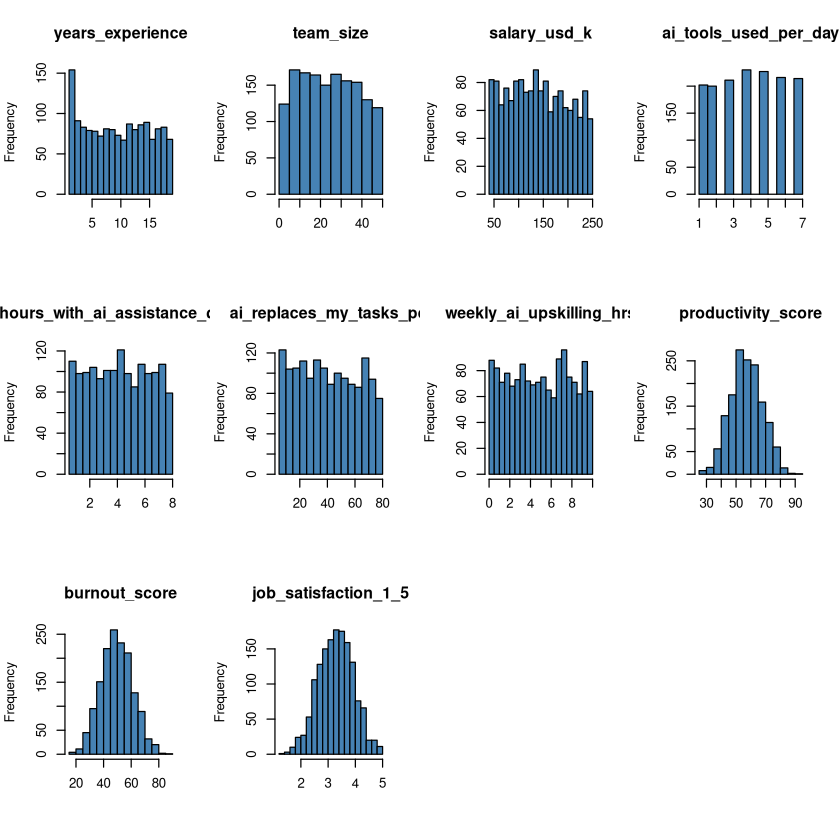
\includegraphics[width=\textwidth, height=0.68\textheight, keepaspectratio]{histograms}
    \end{columns}
\end{frame}

\begin{frame}{Correlations between Variables}
    \begin{center}
        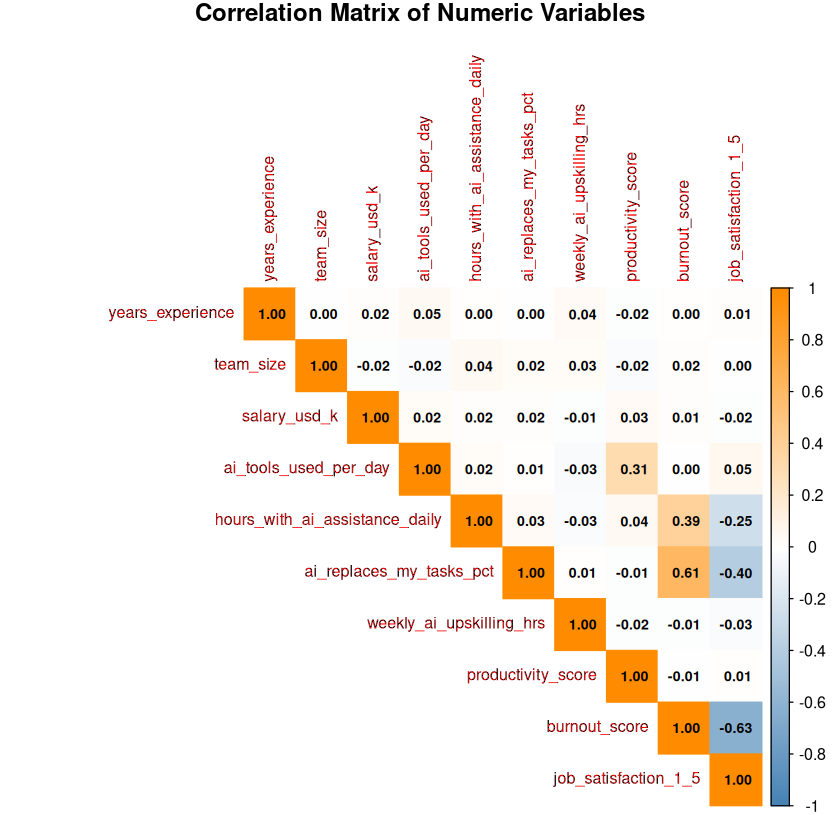
\includegraphics[width=0.72\textwidth, height=0.78\textheight, keepaspectratio]{correlation}
    \end{center}
\end{frame}

%-------------------------------------------------------
\section{Hypothesis}

\begin{frame}{Research Question and Hypothesis}
    \textbf{Can we predict burnout score from AI usage and job satisfaction?}
    \vspace{0.6em}
    \begin{block}{Chosen predictors (from correlation analysis)}
        \small
        \begin{itemize}
            \item \texttt{ai\_replaces\_my\_tasks\_pct} -- positive effect \hfill (r = 0.613)
            \item \texttt{job\_satisfaction\_1\_5} -- negative effect \hfill (r = -0.629)
            \item \texttt{hours\_with\_ai\_assistance\_daily} -- positive effect \hfill (r = 0.386)
        \end{itemize}
    \end{block}
    \vspace{0.6em}
    \textbf{Split:} 90\% training (1350 rows) / 10\% test (150 rows)
\end{frame}

\begin{frame}{Predictors vs Burnout Score}
    \begin{center}
        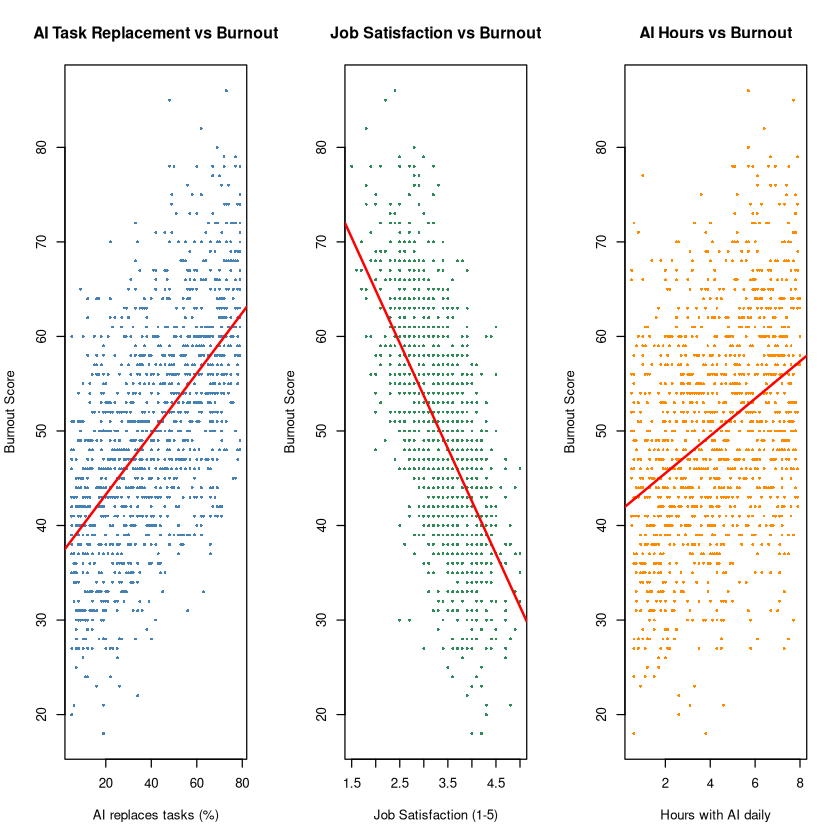
\includegraphics[width=\textwidth, height=0.75\textheight, keepaspectratio]{scatterplots}
    \end{center}
\end{frame}

%-------------------------------------------------------
\section{Model}

\begin{frame}{Linear Regression Model}
    \[
        \hat{y} = 56.75
              + 0.236 \cdot x_{\text{replace}}
              - 6.718 \cdot x_{\text{satisfaction}}
              + 1.418 \cdot x_{\text{hours}}
    \]
    \begin{columns}[c]
        \column{0.42\textwidth}
        \small
        \begin{tabular}{ll}
            \toprule
            Metric & Value \\
            \midrule
            $R^2$ & 0.611 \\
            Adj.\ $R^2$ & 0.610 \\
            Residual SE & 7.10 \\
            F-statistic & 705.2 \\
            p-value & $< 2\text{e-}16$ \\
            \bottomrule
        \end{tabular}
        \column{0.55\textwidth}
        \small
        All three predictors significant at $p < 2\text{e-}16$
        \begin{itemize}
            \item Model explains 61\% of variance in burnout
            \item Strongest predictor: job satisfaction
        \end{itemize}
    \end{columns}
\end{frame}

\begin{frame}{Assumption Checks}
    \begin{center}
        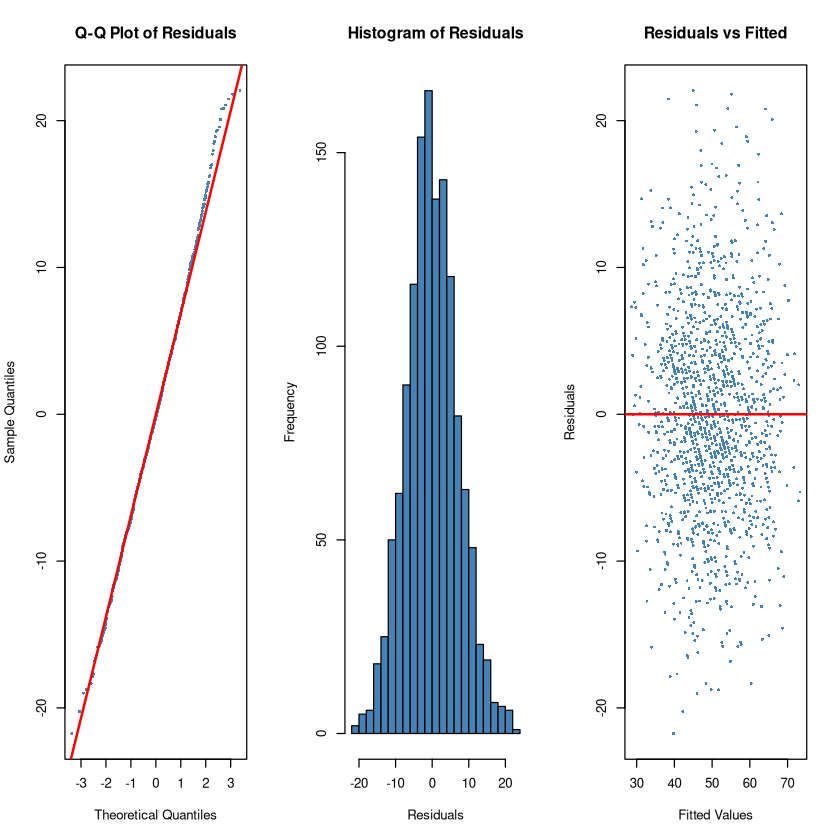
\includegraphics[width=\textwidth, height=0.72\textheight, keepaspectratio]{assumptions}
    \end{center}
    \small Residuals are approximately normal with no systematic pattern.
\end{frame}

%-------------------------------------------------------
\section{Evaluation}

\begin{frame}{Test Set Evaluation}
    \begin{columns}[c]
        \column{0.38\textwidth}
        \small
        \begin{tabular}{ll}
            \toprule
            Statistic & Value \\
            \midrule
            Mean & -0.18 \\
            Std dev & 6.57 \\
            Variance & 43.11 \\
            Min & -19.46 \\
            Max & 14.11 \\
            \bottomrule
        \end{tabular}
        \vspace{0.5em}

        \small Near-zero mean: no bias.\\
        Test SD (6.57) $\approx$ train SE (7.10).
        \column{0.62\textwidth}
        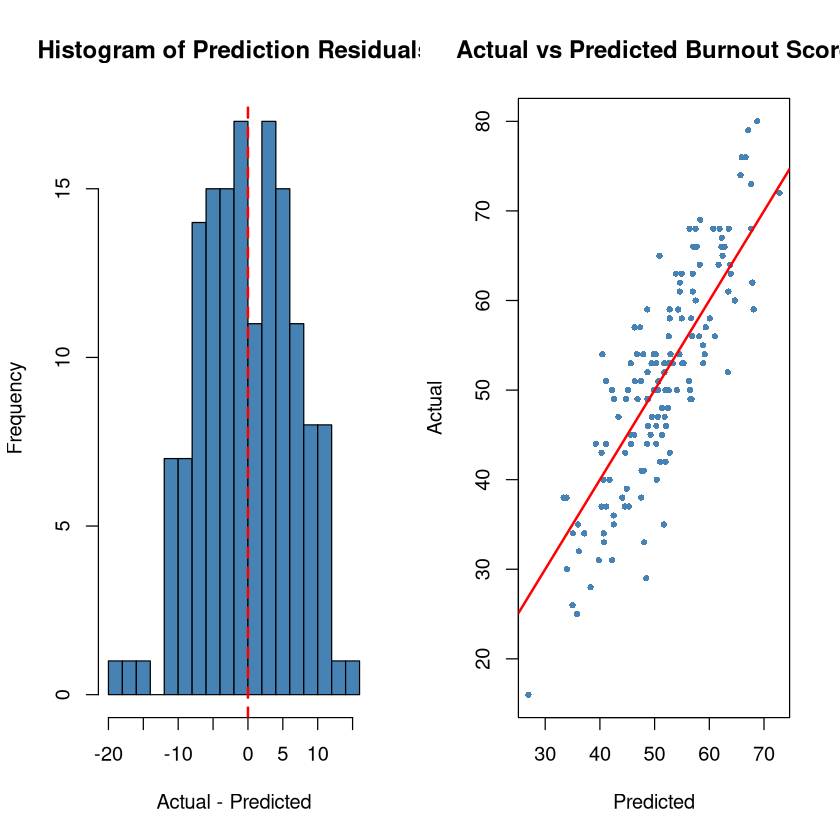
\includegraphics[width=\textwidth, height=0.72\textheight, keepaspectratio]{predictions}
    \end{columns}
\end{frame}

%-------------------------------------------------------
\section{Categorical Analysis}

\begin{frame}{ANOVA: Effect of Categorical Variables on Burnout}
    \begin{columns}[c]
        \column{0.46\textwidth}
        \small
        One-way ANOVA tested five categoricals against \texttt{burnout\_score}:
        \vspace{0.4em}
        \begin{tabular}{lcc}
            \toprule
            Variable & F & p-value \\
            \midrule
            \texttt{attrition\_risk} & \textbf{279.2} & $<2\text{e-}16$ \\
            \texttt{fear\_ai\_repl.} & 1.62  & 0.197 \\
            \texttt{remote\_work}    & 0.94  & 0.391 \\
            \texttt{ai\_adoption}    & 0.47  & 0.703 \\
            \texttt{company\_size}   & 0.21  & 0.934 \\
            \bottomrule
        \end{tabular}
        \vspace{0.5em}

        \small Tukey HSD: all three attrition groups differ at $p < 10^{-6}$
        \column{0.52\textwidth}
        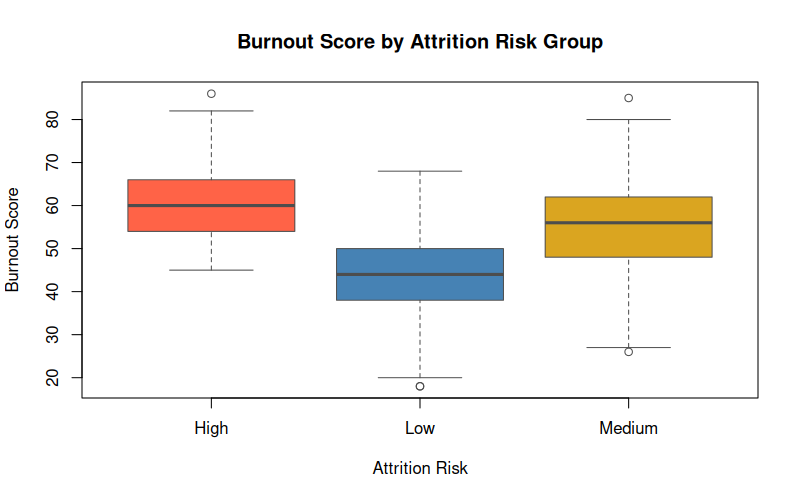
\includegraphics[width=\textwidth, height=0.65\textheight, keepaspectratio]{boxplot_attrition}
    \end{columns}
\end{frame}

\begin{frame}{Chi-Square: Fear of AI and Attrition Risk}
    \begin{columns}[c]
        \column{0.44\textwidth}
        \small
        \textbf{Are fear and attrition independent?}

        $\chi^2 \approx 460$, $\mathrm{df}=4$, $p < 2\text{e-}98$

        \vspace{0.5em}
        Fear distribution within attrition group:
        \vspace{0.3em}
        \begin{tabular}{lccc}
            \toprule
             & Low & Med & High \\
            \midrule
            Low attr.  & 44\% & 46\% & 10\% \\
            Med attr.  & 30\% & 47\% & 23\% \\
            High attr. & 5\%  & 2\%  & \textbf{93\%} \\
            \bottomrule
        \end{tabular}
        \vspace{0.5em}

        \small Fear is a \emph{proxy} for attrition risk, not an independent driver of burnout.
        \column{0.54\textwidth}
        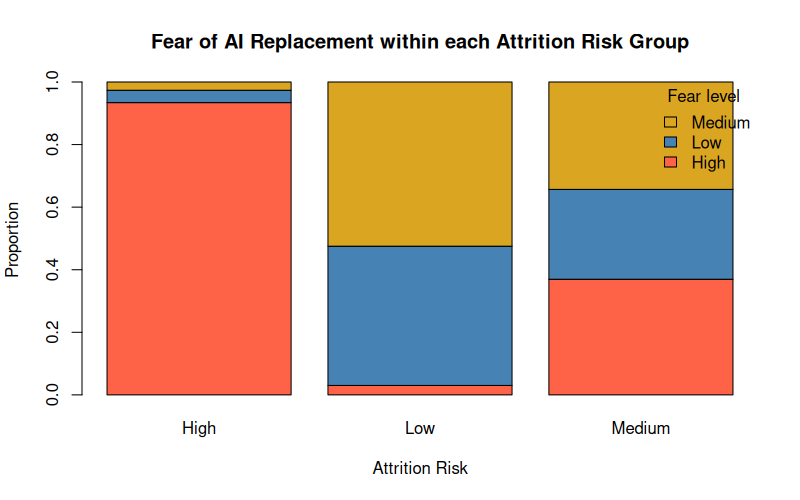
\includegraphics[width=\textwidth, height=0.65\textheight, keepaspectratio]{barplot_fear_attrition}
    \end{columns}
\end{frame}

\begin{frame}{Logistic Regression: Predicting High Attrition Risk}
    \begin{columns}[c]
        \column{0.44\textwidth}
        \small
        Binary outcome: High vs Low/Medium attrition risk

        \vspace{0.4em}
        \textbf{Model:} \texttt{glm(family="binomial")}
        \begin{itemize}
            \item \texttt{burnout\_score} $\uparrow$
            \item \texttt{job\_satisfaction} $\downarrow$
            \item \texttt{fear\_ai} (High) $\uparrow\uparrow$
        \end{itemize}

        \vspace{0.4em}
        \textbf{Test set accuracy: $\approx$95\%}

        \vspace{0.4em}
        \small \texttt{step()} retains all three predictors.\\
        Causal chain:\\
        AI usage $\to$ burnout $\to$ fear $\to$ attrition
        \column{0.54\textwidth}
        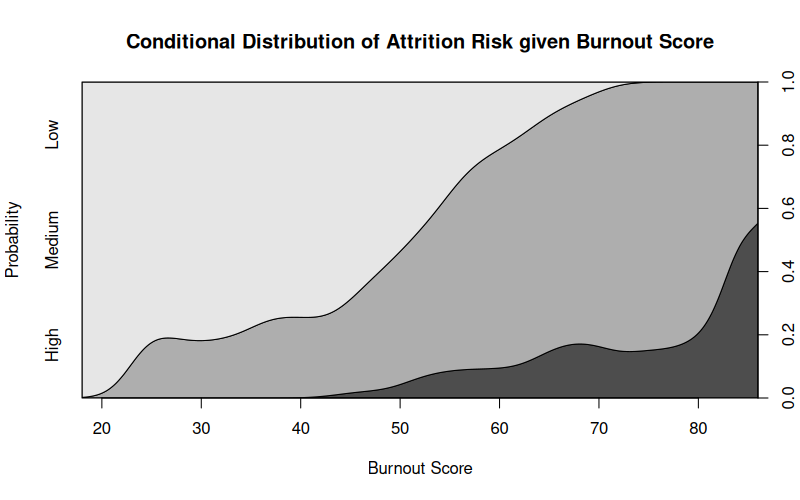
\includegraphics[width=\textwidth, height=0.65\textheight, keepaspectratio]{cdplot_attrition}
    \end{columns}
\end{frame}

%-------------------------------------------------------
\section{Conclusions}

\begin{frame}{Conclusions and Future Paths}
    \begin{columns}[t]
        \column{0.50\textwidth}
        \small
        \textbf{Hypothesis confirmed (Step 3):}
        \begin{itemize}
            \item All 3 predictors significant at $p < 2\text{e-}16$
            \item $R^2 = 0.611$ -- model generalises well
            \item Job satisfaction is the strongest driver
        \end{itemize}
        \vspace{0.4em}
        \textbf{Categorical analysis (Steps 5--7):}
        \begin{itemize}
            \item Only \texttt{attrition\_risk} significant in ANOVA
            \item Fear of AI $\leftrightarrow$ attrition: $\chi^2 \approx 460$
            \item Logistic model: 95\% accuracy on High attrition
            \item \texttt{step()} confirms base model is optimal
        \end{itemize}
        \vspace{0.3em}
        \textbf{Limitation:} cross-sectional data -- causality unestablished
        \column{0.48\textwidth}
        \small
        \textbf{Future paths:}
        \begin{enumerate}
            \item Interaction: replacement \% $\times$ satisfaction
            \item Subgroup models by work type / company size
            \item Longitudinal data for causal inference
            \item Ordinal logistic for all 3 attrition levels
        \end{enumerate}
    \end{columns}
\end{frame}

\end{document}
